\subsection{CMA-ES \label{CMAtheory}}


This section is based on the tutorial written by Nikolaus Hansen
\citep{hansen2011}. The section will not focus on the theoretical derivation
of CMA-ES, but rather how it deviates from Cross Entropy. 
The CMA-ES operates on a general level much like the Cross-entropy 
method, but includes some features that increases the adaptability 
of the algorithm.\\
\\
The CMA-ES, like the Cross Entropy, uses a Gaussian distribution to
search for good solutions to $\fitnessFunction$. Yet, for the 
variance parameter, the CMA-ES provides a full covariance matrix.
As the Cross-entropy method only provides a diagonal matrix of scalers,
it's restricted to only scaling the ellipsoid of equal density along
the coordinate axes. The CMA-ES however, with a full covariance matrix,
allows the ellipsoid to rotate arbitrarily in the search space.\\
Another difference between the two algorithms is that 
Cross-entropy method only considers the next population when updating the
distribution parameters, while the CMA-ES keeps track of 
some information from earlier 
generations. This allows the CMA-ES somewhat keep track of the evolution 
of the sampled vectors.\\
The CMA-ES also differs from the Cross-entropy method in how it evaluates the influence 
of the parent vectors. As the Cross-entropy method weights all vectors equally when 
moving the mean. The CMA-ES, at least from the implementation in Shark, 
has the option of taking a weighted combination of the offspring in order
to bias towards the better vectors.

\begin{figure}[H]
\hrule
\vspace{0.2cm}
{\centering  \textit{CMA-ES}}
\vspace{0.2cm}
\hrule
\begin{algorithmic}
\State{\textbf{input}}
\State{$\fitnessFunction$: The function that estimates the performance of a vector $\individual$}
\State{($\mean$, $C$): The initial mean and variance of the Gaussian distribution, where 
$C$ is the covariance matrix usually set to $C=I$}
\State{$\lambda$: The number of vectors sampled per generation/iteration}
\State{$\offspringNumber$: The number of parents selected for the new mean}
\\
\State{\textbf{initialization}}
\State{Set initial internal parameters}
\\
\Loop
\State{Increment generation counter}
\State{Sample new generation}
\State{Evaluate each vector using $\fitnessFunction$ and recombine}
\State{Covariance matrix adaption}
\State{Step-size control}
\EndLoop
\end{algorithmic}
\hrule
\caption{The pseudo code for the CMA-ES \label{fig:cmaCode}}
\end{figure}

\subsubsection{Input}

\textbf{The objective function} \\
This serves the same purpose as in Cross Entropy (see page \pageref{CEObjective}).
\\

\textbf{The initial mean and variance of the Gaussian distribution} \\
Here $\mean^{(g)}$ is the mean and  
${C^{(g)}}$ is the variance 
of the Gaussian distribution ($\mean^{(g)}$,
${C^{(g)}}$). 
More specifically this Gaussian distribution is defined as 
\begin{align}
\mathcal{N}(\mean^{(\generation)},\sigma^2 C^{(\generation)})
\end{align}

Where $g$ denotes the current iteration/generation.\\


\textbf{The number of vectors}\\
$\populationSize$ is the number of vectors sampled in each generation.
\\

\textbf{The number of parents}\\
$\offspringNumber$ is the number of vectors which are used to compute 
the new mean very much like in the Cross-entropy method. However the CMA-ES algorithm
is not bound to weight each vector equally. It has the option to assign 
a weight to each vector and hence biasing towards the better solutions.
\\


\subsubsection{Initialization}


Set parameters
\begin{align}
\lambda, \offspringNumber, w_{i \dots \offspringNumber}, c_{\sigma}, d_{\sigma}, c_c, c_1, c_{\offspringNumber}
\end{align}
To their default values according to table 1 in \citep{hansen2011}.

Set evolution path $p_{\sigma} = 0$, $p_{c} = 0$, covariance matrix $C = I$ and $g = 0$

Where:

\begin{align}
\lambda, \mu, g &\in \mathbb{N}\\
w_i,\dots,w_{\mu}, c_{\sigma}, d_{\sigma}, c_c, c_1, c_{\lambda}, &\in \mathbb{R}\\
p_{c}, p_{\sigma} &\in \mathbb{R}^{\dimensions}\\
C &\in \mathbb{R}^{\dimensions \times \dimensions}
\end{align}

Again, note that $\lambda$ has the meaning of $\populationSize$ from earlier, that
is $\lambda$ is in this case the population size. $\mu$ however, is still the number
of vectors that contribute to the updating of distribution parameters, namely the 
parent size.\\
\\
In this algorithm, the distribution used is multivariate normal distribution defined
as 
\begin{align}
\mathcal{N} \left( m,  \sigma^2 C \right)
\end{align}
This distribution describes the set of correlated real-valued vectors that
clusters around the mean vector $m$ and has a covariance described by the
matrix $C$. The covariance matrix describes the 'shape' of the space in which 
the vectors are most likely to be sampled. For illustrative purposes,
the shape of the sampling space is drawn as an ellipsoid.
This ellipsoid depicts a set of points that has equal density 
in the probability density function of $C$, and is hence referred to 
as the ellipse of equal density.
With a covariance matrix $C$
the ellipsoid is defined as points that satisfies
$\{x \in R^{\dimensions} | x^{T} C^{-1} x = 1\}$.
When illustrating this, the step-size is set as $\sigma = 1$ for simplicity.\\
\\
The matrix $C^{-1}$ is decomposed as $C^{-1} = B D^{-2} B^T$, where $B$ is a rotation 
matrix that rotates from the coordinate axes into the principal axes of $C$, and 
$D^{-2}$ is the diagonal matrix 
$\text{diag} \left( \frac{1}{d_{1}^2},\dots, \frac{1}{d_{\dimensions}^2} \right)$
where $d_{i}$ is the $i$'th eigenvalue of $C$. Figure \ref{fig:ellipse} shows an example
of how to determine if a point lies on the ellipsoid. In this example, the aim is to 
determine if the point $x$ lies on the two-dimensional ellipsoid, hence checking if 
$x^{T} C^{-1} x = 1 \Leftrightarrow x^{T} B D^{-2} B^T x = 1 $ holds. In figure 
\ref{fig:ellipse}, $l$ is the length from the origin of the ellipse to the edge.
Consider the operation
\begin{align}
B D^{-2} B^T x \label{eq:rotscal}
\end{align}

The order of operations are the following. 
$B^{T}$ rotates $x$ from the principal axises of $C$
into the coordinate axises. Then $D^{-2}$ scales the point by $\frac{1}{l^2}$ where
$l$ is the length from the ellipsoid origin to the edge. Finally, $B$ rotates the point 
back in the original direction. thus, (\ref{eq:rotscal}) has the same effect as
\begin{align}
\frac{1}{l^2} x
\end{align}
Hence, the entire operation is equivalent to
\begin{align}
x^{T} B D^{-2} B^T x &= x^{T} \frac{1}{l^2} x = \frac{1}{l^2} x^{T} x
= \frac{1}{l^2} ||x||^2
\end{align}
This means that if $||x||^2 = l^2$ then $x$ lies on the ellipse.
In the example of figure \ref{fig:ellipse}, $x$ is not 
on the ellipse.


\begin{figure}[H]
\begin{center}

\end{center}
\begin{center}
\ellipseFigure
\end{center}
\caption{Illustration of $\{x \in R^{\dimensions} | x^{T} C^{-1} x \stackrel{?}{=} 1\}$ \label{fig:ellipse}}
\end{figure}

\subsubsection{Loop}

\textbf{Increment iteration counter}

If the stopping criteria is not met, then
\begin{align}
g &= g+1
\end{align}
Otherwise, stop.\\


\textbf{Sample new generation}\\
Sample new population of search points, for $k = 1, \dots, \lambda$.
The aim is to sample vectors in the following form
\begin{align}
\individual_{k} \sim \mathcal{N}(m, \sigma^2 C)
\end{align}


To generate the sample for the generation, the covariance matrix is first 
decomposed using principal component analysis into
\begin{align}
C = B D^2 B^{T}
\end{align}

Where $B = \begin{bmatrix}
b_1, & \dots, & b_\dimensions
\end{bmatrix}$ 
is am orthogonal basis of eigenvectors, and  
$D = \text{diag}\left(d_1, \dots, d_\dimensions\right)$
is a diagonal matrix that contains all eigenvalues of $C$.\\
\\
Intermediately, the vectors are sampled from a Gaussian distribution 
with a mean of zero and
the identity matrix as variance
\begin{align}
z_{k} &\sim \mathcal{N}(0, I)
\end{align}

$z_k$ is then multiplied by a factor that causes the them to form 
after the covariance matrix $C$. From Hansens tutorial, it's derived that
\begin{align}
C^{-1} &= B D^{-2} B^{T}\\
C^{\frac{1}{2}} &= B D B^{T}
\end{align}

Thus, to get the effect of the covariance matrix to apply to the $z_k$
samples, the following is used

\begin{align}
\mathcal{N}\left( 0, C \right) \sim C^{\frac{1}{2}} \mathcal{N}\left( 0, I \right)
\end{align}

\begin{align}
y_{k} &= B D \underbrace{B^{T} z_{k}}_{\sim \mathcal{N}(0, I)} \sim \mathcal{N}(0, C)\\
y_{k} &= B Dz_{k} \sim \mathcal{N}(0, C) \label{eq:sampley}
\end{align}

$B$ is the orthogonal basis of vectors of unit length, which means that 
$B$ is purely a rotation matrix. Due to this, $B^{T} z_{k}$ only rotates
$z_k$ yielding the same distribution. After this, the $BD$ is multiplied,
which applies the scale such that each vector is scaled to match the
variance in the principal axises of the covariance matrix, and $B$ 
will rotate each sample such that it aligns with the principal axises
of $C$. After this step, $y_{k}$ now resemble the vectors that rotated and scaled
to match shape of the covariance matrix.\\

The mean and step-size $\sigma$ is applied.
\begin{align}
x_{k} &= m + \sigma y_{k} \sim \mathcal{N}(m, \sigma^2 C) \label{eq:finalSample}
\end{align}



Finally, the $x_{k}$ vector resemble a realization of the Gaussian distribution
with mean $m$ and covariance matrix $C$ scaled by the step-size $\sigma$.
Am illustration of the sampling process in two dimensions can be seen in figure \ref{fig:sampleing}, where 
\begin{align}
\sigma = 1,\ B = \begin{bmatrix}
{b_1}_x & {b_2}_x\\
{b_1}_y & {b_2}_y
\end{bmatrix},\ D = \begin{bmatrix}
d_1 & 0\\
0   & d_2
\end{bmatrix}
\end{align}


\begin{figure}[H]
\begin{center}
\begin{tabular}{c c c}
\begin{tikzpicture}[scale=0.5]
\draw [->] (0,-5) -- (0,5);
\draw [->] (-5,0) -- (5,0);
\node at (0,0) {};
\draw  (0,0) ellipse (2 and 2);
\draw (0,0) -- (2,0);
\draw [decorate,decoration={brace,amplitude=5,raise=2},yshift=0pt]
(0,0) -- (2,0) node [black,midway,xshift=0,yshift=15] {1};
\end{tikzpicture} &
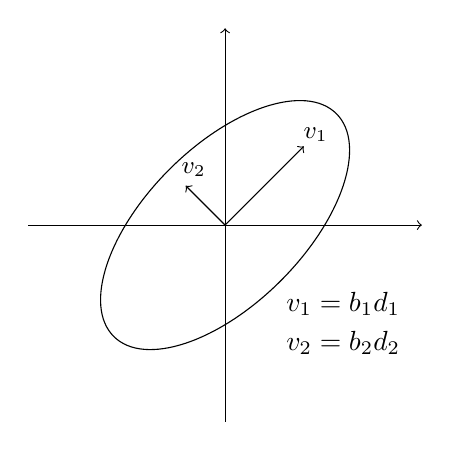
\begin{tikzpicture}[scale=0.5]
\draw [->] (0,-5) -- (0,5);
\draw [->] (-5,0) -- (5,0);
\node at (0,0) {};
\draw [rotate=45] (0,0) node (v1) {} ellipse (4 and 2);
\draw [->] (0,0) --  (2,2);
\draw [->] (0,0) -- (-1,1);
\node at (-0.8,1.4) {\small $v_2$};
\node at (2.3,2.3) {\small $v_1$};
\node at (3,-2) {$v_1 = b_1 d_1$};
\node at (3,-3) {$v_2 = b_2 d_2$};
\end{tikzpicture} &
\begin{tikzpicture}[scale=0.5]
\draw [->] (0,-5) -- (0,5);
\draw [->] (-5,0) -- (5,0);
\node at (1,1) {};
\draw [rotate=45] (1.5,0) node (v1) {} ellipse (4 and 2);
\draw [->](1,1) -- (3,3);
\draw [->] (1,1) -- (0,2);
\draw [fill] (1,1) ellipse (0.1 and 0.1);
\node at (2,1) {\small $m$};
\end{tikzpicture}\\
$z_{k} \sim \mathcal{N}(0, I)$ & $y_{k} \sim B Dz_{k}$ & $x_{k} \sim m + \sigma y_{k} \sim \mathcal{N}(m, \sigma^2 C)$
\end{tabular}
\end{center}
\caption{The steps of the sampling process \label{fig:sampleing}}
\end{figure}
In the middle step, the CMA-ES algorithm differs in particular from the Cross-entropy method
as the rotation matrix $B$ is applied and rotates the distribution shape. 
In opposition to this, the Cross-entropy method distribution is aligned with
the coordinate system axises.\\

\textbf{Evaluate each vector using $\fitnessFunction$ and recombine}\\
As each vector is evaluated, they are ranked such that
$\fitnessFunction{ \left( \individual_{i} \right) } \geq \dots \geq \fitnessFunction{ \left( \individual_{\offspringNumber} \right)} \geq \dots \geq \fitnessFunction{ \left( \individual_{\lambda} \right)}$.

\begin{align}
\langle y \rangle_{w} &= \sum^{\offspringNumber}_{i = 1}w_{i} y_{i : \lambda}
\end{align}

Where the notion of $y_{i : \lambda}$ means the $i$'th element in ranked list of vectors
where $y_1$ is the best ranked vector.

\begin{align}
\sum^{\offspringNumber}_{i = 1} w_{i} = 1, w_{i} > 0
\end{align}

$\langle y \rangle_{w}$ is a measure of a 'weighted center of mass',
and is part of the selection mechanism. The idea is to allow the selected vectors
to contribute differently to the update, and hence emphasize the higher 
ranking vectors. The individual weights are as the following

\begin{align}
w_i &= \frac{w_{i}'}{\sum^{\offspringNumber}_{j=1} w_j }
\end{align}

Where the $w_i'$ is used for a intermediate weighting value for the vectors.\\
In the Shark library, three built-in weighting types are implemented, each with
a distinct intermediate weight.

\begin{align}
\text{Equal}: &\quad w_i' = 1 \label{eq:recomType}\\
\text{Linear}: &\quad  w_i' = \offspringNumber - i\\
\text{Superlinear:} &\quad w_i' = ln \left( \offspringNumber + \frac{1}{2} \right)
- ln \left( i \right)
\end{align}
Thus, with the equal, each vector contributes equally, and with the other two, the 
higher ranking vectors has more influence on location of the 'center of mass' of 
the selection.

The new mean is computed as
\begin{align}
m^{(g+1)} &= m^{(g)} + \sigma \langle y \rangle_{w} = \sum^{\offspringNumber}_{i = 1} w_{i}x_{i:\lambda} \label{eq:movemean}
\end{align}
Such that the mean moves towards the 'center of mass' scaled by the step-size.
The details of step-size $\sigma$ is covered later in this section,
however in brief terms the step-size is meant to scale movements 
of the mean and the distribution area.\\
\\
In relation to the selection mechanism, the value $\mu_{eff}$ is introduced.
This is defined as
\begin{align}
\meff = \left( \sum_{i=1}^{\offspringNumber} w_i^2 \right)^{-1}
\end{align}
Hence $1 \leq \meff \leq \mu$. As an example, for the equal recombination
type, $\meff = \left( \sum_{i=1}^{\offspringNumber} w_i^2 \right)^{-1} = 1^{-1} =1$
In the tutorial by N. Hansen, it's mentioned that $\meff \approx 
\frac{\lambda}{4}$ indicates a good setting of $w_i$. The $\meff$ is 
measure of how much of the parent mass is used, and serves as a normalization 
factor in later equations.\\

\textbf{Covariance matrix adaption}

The idea of using the covariance matrix is to make new samples
resemble the covariance of the previous well-performing vectors, as opposed 
to the Cross-entropy method that does not maintain any information of
previous samples.\\
\\
A evolution path of the movement of the means is introduced as $p_{c}$. This 
is a vector that holds the direction in which the mean has been moved in 
both the current generation, and in previous generations in 
a 'low-pass filter' like manner. Using the 
evolution path, the covariance matrix can take a shape that 
makes samples more likely to appear in the direction of successive 
movements of the mean.
The evolution path for generation $g+1$ is updated as



\begin{align}
p_{c}^{(g+1)} &= \underbrace{\left( 1 - c_{c} \right) 
p_{c}^{(g)}}_{\makebox[0pt]{\text{previous steps}}}  + 
\overbrace{h_{\sigma}}^{\makebox[0pt]{\text{{indicator function}}}}
\underbrace{\sqrt{c_{c} \left( 2 - c_{c} \right) \offspringNumber_{\text{eff}}}}_{
\makebox[0pt]{\text{normalization}}
}
\langle y \rangle_{w} \label{eq:epathc}
\end{align}
In (\ref{eq:epathc}), the term $\left( 1 - c_{c} \right) p_{c}^{(g)}$ makes 
the evolution path become influenced by earlier path steps. The learning rate
$c_c \in [0;1] $ indicates how much of the previous path is taken into account.
if $c_c = 0$, the previous path is not considered at all, and if $c_c = 1$ the path 
will only consist of the previous step. According to the tutorial, this is set
$c_c = \frac{4 + \mu_{eff} / \dimensions}{\dimensions + 4 + 2 \mu_{eff} / \dimensions}$.\\
\\
The indicator function $h_{\sigma}$ is discussed in detail in the tutorial \citep{hansen2011}.
However, the main idea of this indicator function is.
\begin{align}
h_{\sigma}
\begin{cases} 1\ \ \ \text{if $||p_{\sigma}||$ is large} \\
              0\ \ \ \text{otherwise} %
\end{cases}
\end{align}
The purpose of this is to stall updating the evolution path when 
the length of the step-size evolution path becomes too large. The step-size
evolution path is covered in \textit{Step-size control}.\\
\\
The normalization factor 
$\sqrt{c_{c} \left( 2 - c_{c} \right) \offspringNumber_{\text{eff}}}$ is chosen such that
$p^{(g+1)}_{c} \sim \mathcal{N}\left(0, C \right)$ if $p_c^{(g)} \sim \mathcal{N} 
\left(0, C\right)$\\
To see that this holds, note the following
\begin{align}
\langle y \rangle_{w} &= \frac{m^{(g+1)} - m^{(g)}}{\sigma}
\sim \frac{1}{\sqrt{\meff}}  \mathcal{N}\left(0, C \right)
\end{align}
\\
Thus, with the indicator function set aside
\begin{align}
p_{c}^{(g+1)} &\sim \left( 1 - c_{c} \right) 
\mathcal{N}\left(0, C \right) + 
\sqrt{c_{c} \left( 2 - c_{c} \right) \offspringNumber_{\text{eff}}}
\frac{1}{\sqrt{\meff}}\mathcal{N}\left(0, C \right) \label{eq:nomalization_start}\\
&\sim
\mathcal{N}\left(0, \left( 1 - c_{c} \right)^2 C \right) + 
\mathcal{N}\left(0, c_{c} \left( 2 - c_{c} \right)  C \right)\\
&\sim
\mathcal{N}\left(0, \left( 1 - c_{c} \right)^2 C + c_{c} \left( 2 - c_{c} \right)  C  \right)\\
&\sim \mathcal{N}\left( 0, C \right) \label{eq:nomalization_end}
\end{align}
Hence, the evolution path is updated unbiased under random selection.
\\
The covariance matrix is updated as follows
\begin{align}
C^{(g+1)} &= 
\underbrace{\left( 1 - c_{1} - c_{\offspringNumber} \right)C^{(g)}}_{
\makebox[0pt]{\text{{smoothing of previous steps}}}
} + 
\overbrace{c_{1} \left( p_{c}^{(g+1)} {p_{c}^{(g+1)}}^{T}\right)}^{
\makebox[0pt]{\text{{Rank-one update}}}
} +
\underbrace{c_{\offspringNumber} \sum^{\offspringNumber}_{i = 1} w_{i} y_{i : \offspringNumber} y_{i : \offspringNumber} ^{T}}_{
\makebox[0pt]{\text{{Rank-$\mu$ update}}}
} \label{eq:fullCMA}
\end{align}

Again, the first term is the smoothing of the previous covariance matrices.
the constants $c_1$ and $c_\mu$ are the learning rates for respectively the two
different updates, and the sum of them must not exceed 1, $c_1 + c_\mu \leq 1$.\\
\\
The rank-one update is meant to form the covariance matrix in a way such that 
it becomes more likely for the distribution to draw vectors in the direction of
successive steps. The term 
\begin{align}
c_{1} \left( p_{c}^{(g+1)} {p_{c}^{(g+1)}}^{T}\right)
\end{align}
is first of all factored by the leaning rate $c_1$. The matrix computed as 
$p_{c}^{(g+1)} {p_{c}^{(g+1)}}^{T}$ is the outer product of the evolution path. 
Remember here that the $p_{c}^{(g+1)}$ is the smoothed vector that indicates 
the path in which the mean has been moved. Hence, the covariance will for this 
single vector be purely in the direction of the mean's movement. Also, as it's 
the outer product of just one vector, the rank of this matrix is one, hence the
name 'rank-one update'.\\
\\
The last term in (\ref{eq:fullCMA}) namely the rank-$\mu$ update
\begin{align}
c_{\offspringNumber} \sum^{\offspringNumber}_{i = 1} w_{i} y_{i : \offspringNumber} y_{i : \offspringNumber} ^{T} \label{eq:rankmuupdate}
\end{align}
Again, the entire term is factored by the learning rate $c_\mu$. The sum
of outer products yields and estimate for the covariance matrix of the vectors
sampled as $y_{i : \offspringNumber} \sim \mathcal{N}\left(0, C^{(g)}\right)$ 
(see (\ref{eq:sampley})). Thus (\ref{eq:rankmuupdate}) corresponds to the 
estimated covariance of the best selected vectors, with a weighting factor
such that the covariance of the highest ranking vectors may contribute the most.
The rank of the matrix in \ref{eq:rankmuupdate} is $min(\mu, \dimensions)$.\\
\\
As a result of this, when the covariance matrix is updated as in (\ref{eq:fullCMA})
the next sample will be more likely to be realized somewhat like the previous 
samples, somewhat in the direction in which the mean was moved and somewhat 
according to the covariance of the highest ranking vectors.
\\



\textbf{Step-size control}

In the CMA-ES algorithm, the step-size $\sigma$ is used as an isotropic scale across
each of the principal axes in the covariance matrix. Hence the stepsize is used as 
an 'overall' scaling mechanism when drawing vectors. The step-size is used when 
sampling the vectors in (\ref{eq:finalSample}) where it expands the variance 
of the distribution. When moving the mean in (\ref{eq:movemean}), the weighted 
selection mass \textbf{scaled} with the step-size is added to the mean.

First we consider the evolution path of the step-size $p_\sigma$ which is
updated as follows.

\begin{align}
p_{\sigma}^{(g+1)} &= 
\underbrace{\left( 1 - c_{\sigma} \right) p_{\sigma}^{(g)}}_{
\makebox[0pt]{\text{{smoothing of previous steps}}}
}
+ 
\overbrace{\sqrt{c_{\sigma} \left( 2 - c_{\sigma} \right) \meff}}
^{
\makebox[0pt]{\text{{normalization}}}
} 
\underbrace{C^{- \frac{1}{2}}}_{
\makebox[0pt]{\text{{scale/rotation}}}
}
\langle y \rangle_{w}
\end{align}
The first term is the smoothing step as seen before, only using the learning rate 
associated with the step-size evolution path, but is similar to what is seen in
(\ref{eq:epathc}). The normalization constant is also very similar to the
equivalent factor in (\ref{eq:epathc}).\\
\\
A newly introduced factor is the $C^{-\frac{1}{2}}$ with the decomposition
$C^{-\frac{1}{2}} = B D^{-1} B^{T}$ which has the following effects. $B^{T}$
rotates the principal axises to align with the coordinate axises. 
$D^{-1}$ scales the axises into equal size, and finally, $B$ rotates the 
axises back into the original direction. The transform $C^{-\frac{1}{2}}$
has the effect of making the length of the $p_\sigma$ independent of 
direction as each dimension is normalized.\\
\\
The final effect is that
\begin{align}
p_\sigma^{(g+1)} &\sim \mathcal{N}\left(0, I \right)\\
\text{When }
p_\sigma^{(g)} &\sim \mathcal{N} \left(0, I \right)
\end{align}
With almost the same steps as (\ref{eq:nomalization_start}) through 
(\ref{eq:nomalization_end}).
\begin{align}
p_\sigma^{(g+1)} &\sim (1 - c_\sigma) \mathcal{N}\left( 0, I \right) + \sqrt{c_\sigma 
\left( 2-c_\sigma \right)\meff } {C^{(g)}}^{-\frac{1}{2}} \frac{1}{\sqrt{\meff}}
\mathcal{N} \left( 0, C^{(g)} \right)\\
&\sim \mathcal{N} 
\left( 
  0, 
  \left(  
    \left( 
      1-c_\sigma 
    \right)^2 + \sqrt{c_\sigma 
    \left(  
      2 - c_\sigma
    \right)}^2
  \right) I
\right) \sim \mathcal{N} \left( 0, I \right)
\end{align}

Hence, under random selection, the evolution path $p_\sigma \sim \mathcal{N} 
\left( 0, I \right)$.  The step-size is adapted by comparing the length
if the evolution path $||p_\sigma||$ with the expected length of a vector 
drawn from $\mathcal{N} \left( 0, I \right)$, that is
$\mathbb{E}||\mathcal{N}\left(0, I\right)||$. where 
$\mathbb{E}||\mathcal{N}\left(0, I\right)|| \approx \sqrt{n} + \mathcal{O}\left(1/n\right)$
The cases if this comparison are:

\begin{align}
\textbf{a: } ||p_\sigma^{(g+1)}|| &> \mathbb{E}||\mathcal{N}\left(0, I\right)|| 
\label{case1}\\
\textbf{b: } ||p_\sigma^{(g+1)}|| &< \mathbb{E}||\mathcal{N}\left(0, I\right)||
\label{case2}\\
\textbf{c: } ||p_\sigma^{(g+1)}|| &= \mathbb{E}||\mathcal{N}\left(0, I\right)||\label{case3}
\end{align}
In case \textbf{a} the steps are correlated and the idea is that a larger step-size
would cause the mean to move towards a desired location faster. In case \textbf{b},
the path is short and/or anti correlated. This means that the algorithm would benefit from
shorter steps, and therefore decrease the step-size. In the final case \textbf{c}, the 
steps appear perpendicular and the step-size appears reasonable.
\begin{figure}[H]
\begin{center}
\begin{tabular}{c c c}
\begin{tikzpicture}[scale=0.5]
\draw (0,0) rectangle (8,8);

\draw[-{Triangle[angle=45:5pt 5]}]  (2.1179,1.9813) --  (3.1724,2.5788);
\draw[-{Triangle[angle=45:5pt 5]}]   (3.1724,2.5788) -- (4.2972,2.4734) ;
\draw[-{Triangle[angle=45:5pt 5]}] (4.2972,2.4734)  --  (5.0705,3.1061);
\draw[-{Triangle[angle=45:5pt 5]}] (5.0705,3.1061) -- (5.0705,4.266)  ;
\draw[-{Triangle[angle=45:5pt 5]}](5.0705,4.266)   -- (6.1601,4.969);
\draw[-{Triangle[angle=45:5pt 5]}] (6.1601,4.969) --  (5.5626,7.1131);

\draw[-{Triangle[angle=45:5pt 5, open]}]  (2.1179,1.9813) ->  (5.5626,7.1131);
\end{tikzpicture} &
\begin{tikzpicture}[scale=0.5]
\draw (0,0) rectangle (8,8);

\draw[-{Triangle[angle=45:5pt 5]}] (2.1179,1.9813) -- (2.6803,3.9496);
\draw[-{Triangle[angle=45:5pt 5]}] (2.6803,3.9496) -- (1.0986,3.9145);
\draw[-{Triangle[angle=45:5pt 5]}] (1.0986,3.9145) -- (0.7119,2.0867);
\draw[-{Triangle[angle=45:5pt 5]}] (0.7119,2.0867) -- (2.3288,0.7511);
\draw[-{Triangle[angle=45:5pt 5]}] (2.3288,0.7511) -- (3.8402,1.8758);
\draw[-{Triangle[angle=45:5pt 5]}] (3.8402,1.8758) -- (3.2427,2.7194);

\draw[-{Triangle[angle=45:5pt 5, open]}] (2.1179,1.9813)-> (3.2427,2.7194);
\end{tikzpicture} &
\begin{tikzpicture}[scale=0.5]
\draw (0,0) rectangle (8,8);

\draw[-{Triangle[angle=45:5pt 5]}] (2.1179,1.9813) -- (3.559,2.2976) ;
\draw[-{Triangle[angle=45:5pt 5]}]  (3.559,2.2976)  --  (2.6452,3.6684);
\draw[-{Triangle[angle=45:5pt 5]}]  (2.6452,3.6684) --  (4.6487,3.2115);
\draw[-{Triangle[angle=45:5pt 5]}]  (4.6487,3.2115) --  (5.914,4.266) ;
\draw[-{Triangle[angle=45:5pt 5]}]  (5.914,4.266)  -- (6.0195,5.918) ;
\draw[-{Triangle[angle=45:5pt 5]}] (6.0195,5.918)  --  (4.5784,6.0938);

\draw[-{Triangle[angle=45:5pt 5, open]}] (2.1179,1.9813) ->  (4.5784,6.0938);
\end{tikzpicture}\\
\textbf{a} Correlated steps &
\textbf{b} Anti-correlated steps &
\textbf{c} Uncorrelated steps
\end{tabular}
\end{center}
\caption{Illustratio of evolution path cases \label{fig:evolutionPath}}
\end{figure}

Eventually, the step-size is updated by the following
\begin{align}
\sigma^{(g+1)} &= \sigma^{(g)} \cdot exp \left( \frac{c_{\sigma}}{d_{\sigma}} \left( \frac{||p_\sigma^{(g+1)}||}{E|| \mathcal{N}(0, I) ||} - 1 \right) \right)
\end{align}
Where $0 \leq \frac{c_\sigma}{d_\sigma} \leq 1$ is a damping factor for step-size changes.
This update of the step-size will scale the step-size unbiased in direction 
according to the cases in 
(\ref{case1}), (\ref{case2}) and (\ref{case3}).









